\chapter{The Container Loading Problem}
\section{Formal Problem Definition}
\section{Computational Complexity and NP-hardness}

The placement and assignment of three-dimensional items to larger, mostly rectangular
containers, is a well known problem in logistics and operations research, as the
potential of cost savings and efficiency gains is substantial by reducing the number
of needed containers or by fulfilling customer needs. \gls{CLP} problems are differentiated
by \cite{bortfeldt_constraints_2013} in \textit{input minimization}, where the number
of needed containers is minimized, and \textit{output maximization} problems, where the
value of the associated items is maximized. So, is the \gls{BPP} belonging
to \textit{input minimization} problems, and the \gls{KP} to \textit{output maximization}.

Apart from the expected outcome of the optimization, the characterics of the items
and containers is relevant for the problem definition. Items can be either homogenous or heterogenous,
where homogenous items are identical in size and shape, and heterogenous items are
different in size and shape. The container is usually defined as a three-dimensional space
with a fixed size and shape, where the items have to be placed in \parencite{bortfeldt_constraints_2013}.
Other - non rectangular - shapes are scarcely considered in the literature, as the practical relevance is
limited \parencite{bortfeldt_constraints_2013}. Multiple containers, with homogeneous
or heterogenous size,  are used, whenever the volume and weight of the items requires it.
A possible placement of cargo into a container can be seen in Figure \ref{fig:solution-visualization}.
%Hier angeben welcher Typ betrachtet wird? 

\begin{figure}[ht]
    \centering
    \includegraphics[width=7cm]{pictures/3l_cvrp_example.png}
    \caption{Visualization from \cite{tamke_branch-and-cut_2024}.}
    \label{fig:solution-visualization}
\end{figure}

\section{Constraints in the CLP}
The placement of items is not sufficient, if there is a possible packing
of the items, but practical requirements are not met according to \cite{bischoff_issues_1995}.
Based on the original impulse of \cite{bischoff_issues_1995}, \cite{bortfeldt_constraints_2013}
have systemized all constrains relevant for the \gls{CLP} in five groups.
\begin{itemize}
    \item[1] Container related constraints
    \item[2] Item related constraints
    \item[3] Cargo related constraints
    \item[4] Positioning constraints
    \item[5] Load related constraints
\end{itemize}

% Hier die constriants hinzufügen, die immer gelten, 
% items immer parallel zu wänden gepackt und so 



\subsubsection{Container related constraints}
These constraints summarize all physical barriers of the container, including
the accumulated \textbf{weight} and \textbf{volume} of the cargo. These two
constraints are usually found in the \gls{CVRP}. The distribution of the weight
(\textbf{load balance}) plays also an important role for safety reasons, as the
cargo must not move during the transport and the container must not tip over.
In the special case of trucks, uneven axle weight distribution can cause severe
crash consequences \parencite{krebs_advanced_2021}.

\subsubsection{Item related constraints}
Item related constraints define the properties of the item, which are relevant
for the packing. When the container capacity is limited (\textit{output maximization}),
the \textbf{loading priority} constraint can define the priority among possible
item candidates. For each item, which has to be packed, other constraints define
the way how items can be packed. The orientation constraint limits how the item
can be rotated: it can either rotate only around the z-axis or be completely
free to rotate in all directions, with no partial flexibility in between.
When three dimesional packing is considered, the \textbf{stacking} constraint
is relevant for defining which items can be packed on top of each other. \cite{gendreau_tabu_2006}
differentiates between \textit{fragile} and \textit{non-fragile} items, stating
that non-fragile items can only be stacked on non-fragile items, Figure \ref{fig:stacking_comparison} showcases
this definition. A more sophisticated approach is the calculation  of the
\textit{load-bearing strength} of each box, stating how much pressure the box
can tolerate \cite{krebs_advanced_2021}.

\begin{figure}[htbp]
    \centering
    % First TikZ picture
    \begin{subfigure}[b]{0.45\textwidth}
        \centering
        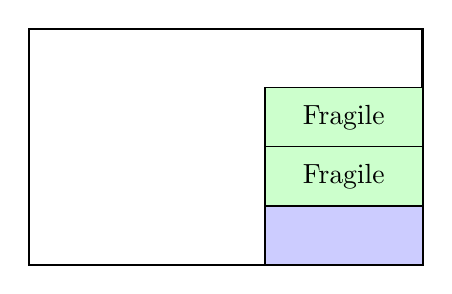
\begin{tikzpicture}
            % Draw the container
            \draw[thick] (0,0) rectangle (5,3);

            % Draw the three items inside
            \draw[fill=blue!20] (3,0) rectangle (5,0.75);
            \node at (4, 0.5) {};

            \draw[fill=green!20] (3,0.75) rectangle (5,1.5);
            \node at (4, 1.125) {Fragile};

            \draw[fill=green!20] (3,1.5) rectangle (5, 2.25);
            \node at (4, 1.875) {Fragile};

        \end{tikzpicture}
        \caption{Feasible stacking of items}
    \end{subfigure}
    \hfill
    % Second TikZ picture
    \begin{subfigure}[b]{0.45\textwidth}
        \centering
        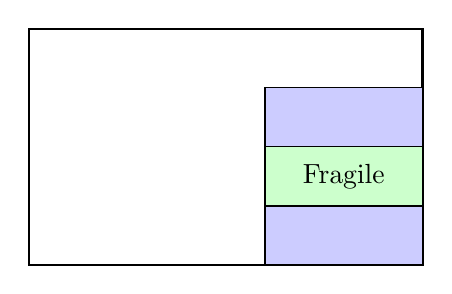
\begin{tikzpicture}
            \draw[thick] (0,0) rectangle (5,3);

            % Draw the three items inside
            \draw[fill=blue!20] (3,0) rectangle (5,0.75);
            \node at (4, 0.5) {};

            \draw[fill=green!20] (3,0.75) rectangle (5,1.5);
            \node at (4, 1.125) {Fragile};

            \draw[fill=blue!20] (3,1.5) rectangle (5, 2.25);
            \node at (4, 1.875) {};
        \end{tikzpicture}
        \caption{Infeasible stacking of items}
    \end{subfigure}
    \caption[Visualization fragile stacking]{Comparison fragile stacking \footnotemark}
    \footnotetext{Own figure}
    \label{fig:stacking_comparison}
\end{figure}

